\documentclass[conference,final]{IEEEtran}

\usepackage{graphicx}
\usepackage{epsfig}
\usepackage{subfigure}
\usepackage[hypertex]{hyperref}
\usepackage{subfigure}  
\usepackage{color}
% \usepackage{draftcopy}

\usepackage[small,it]{caption}

\usepackage{multirow}
\usepackage{ifpdf}

% \newcommand{\jha}[1]{\textcolor{red}{\bf Jha:} }
% \newcommand{\hartmut}[1]{\textcolor{blue}{\bf Hartmut} }
% \newcommand{\yaakoub}[1]{\textcolor{green}{\bf Yaakoub} }
% \newcommand{\ole}[1]{\textcolor{red}{\bf Ole} }

\newcommand{\jha}[0]{}
\newcommand{\hartmut}[0]{}
\newcommand{\andre}[0]{}
\newcommand{\ole}[0]{}

\newcommand{\fixme}[1]{ { \bf{ ***FIXME: #1 }} }
\newcommand{\jhanote}[1]{ {\textcolor{red} { ***Jha: #1 }}}
%\newcommand{\jhanote}[0]{}
\newcommand{\jitter}[1]{{$\sigma(\alpha)$}}

\newif\ifpdf
\ifx\pdfoutput\undefined
  \pdffalse
\else
  \ifnum\pdfoutput=1
    \pdftrue
  \else
    \pdffalse
  \fi
\fi

\ifpdf
\DeclareGraphicsExtensions{.pdf, .jpg}
\else
\DeclareGraphicsExtensions{.eps}
\fi


\begin{document}


\title{\large Application Level Inter-operability Using  SAGA}

% \author{\authorblockN{Shantenu Jha\authorrefmark{1}\authorrefmark{2},
%     Hartmut Kaiser~\authorrefmark{1}, Yaakoub El
%     Khamra\authorrefmark{1}, Ole Weidner\authorrefmark{1}}
%   \authorblockA{\authorrefmark{1} Center for Computation and
%     Technology, Louisiana State University, Baton Rouge, 70803}
%   \authorblockA{\authorrefmark{2} Department of Computer Science,
%     Louisiana State University, Baton Rouge, 70803} }

\author{\authorblockN{AnyBody\authorrefmark{1},
     EveryBody\authorrefmark{1}, NoBody\authorrefmark{1},
     SomeBody\authorrefmark{1}}}

\maketitle

\begin{abstract}

Ginpaper by Reidel, discusses applications that are not truly
interoperation across grids. they are what we call grid-unaware
applications. saga enables grid aware applications to establish
interoperabilty.  Saga merges the distinction between interoperation
and interoperabilty.

Discuss Replica-Exchange application. Discuss GridSAT application
Explain why these are grid-applications that require 
interoperability -- which then is not just a nice talking point, but
a necessary feature. 

Interoperation is not sufficient; interoperabilty is necessary.

\end{abstract}

\andre{there is a very important need to have a full long paragraph 
highlighing the connection between the saga job submission and
OGSA-BES.

\begin{keywords}
  eScience Application, Application, Inter-operation, Distributed
  Infrastructure Deployment, Distributed Application Programming,
  Cactus, SAGA,
\end{keywords}

\section{Introduction}

e-Science applications must be able to utilize e-Infrastructure --
whether sophisticated services, or the next generation networks or
customized supercomputers -- to perform better, faster and different
domain specific research~\cite{hey04, hey05}.  The question is how can
we design and develop e-Science applications, that on the one hand are
not limited by the complexity of e-Infrastructure, while on the other
hand are immune to the evolving nature of such infrastructure? 

In other words, how can we compose applications so as to not depend on
the underlying infrastructure -- either in a dynamical sense (ie over
a period of time) or different infrastructure at essentially the same
time.

Interestingly the answer to both is the same: design applications
using well supported standardized interfaces.

\jhanote{Define Application Level Interoperability}

SAGA is a simple high-level programming abstraction that provides some
of these requirements.  It has been compared to the
MPI~\cite{mpiforum_url} for Grid Programming, in that SAGA provides
simplified method calls at the right level of abstraction for the most
commonly required Grid-functionality.  In addition to being simple, an
additional critical feature of SAGA is that it is on the road to
becoming a community standard, thus strengthening the analogy with
MPI.  It is debatable as to when exactly a critical mass of the
community threw their support behind MPI, but irrespective of the
timing, it is clear that the technical merits of MPI coupled with the
fact that it was a community standard played a great role in
increasing the number of applications developed using MPI and the
number of vendors that were willing to support it.

\noindent The primary aim of this paper is to discuss and highlight
SAGA, or for that matter any sufficiently high-level programming
interface with widespread support and commitment to being supported.
as a critical enabling technology for Application-level
interoperability...

Standardization should not be over emphasized but it is critical.

Note it is also stated as the major advantage of OGSA-BES and JSDL in
the ginpaper.


The following are ensuing advantages of proper programming
abstractions, but are not the focus of this current paper.

\noindent {\it Demonstrate the usefulness of SAGA for Grid application
  development:} SAGA provides a high-level programming interface to
Grid functionality, and thus presents arguably, for the first time
ever, the ability to develop complete and sophisticated applications
using simple Grid function calls.  This paper demonstrates the utility
of SAGA for creating applications that can perform across dynamic and
heterogenous infrastructure.

Also worth noting that SAGA is also useful in general for developing
Grid Applications.

In this paper, we report on the development of a network-centric
application using SAGA and Cactus, that is capable of acquiring
application-specific network characteristic data. This data can be
analyzed by the application to dynamically determine the optimal set
of resources to utilize, and having done so is capable of migrating to
the optimal set of resources.  This application can be deployed on any
resource independent of the middleware stack. All that is required is
support for SAGA {\it adaptors} -- the middleware specific glue layer
that enables the middleware to parse the appropriate SAGA function
calls and implement the correct functionality.  As SAGA becomes a
standard~\cite{saga-uc, saga-req, saga-core} there will be increased
willingness on the part of middleware developers and resource
providers to provide these adaptors to the application community.
Additionally, as the deployment of SAGA and required adaptors becomes
wider (pervasive) and deeper (greater functionality), there is an
increased incentive for application developers to use SAGA.


\noindent {\it Integrate SAGA and Cactus:} 

\noindent {\it Utilize the advantages of proper programming
  abstractions:}
Although we focus on a specific application -- gathering network
characteristics for a Poisson Equation solver and migrating the
application -- thanks to the architecture and abstractions used,
similar functionality can be trivially incorporated in more
sophisticated and complex appliations.

\noindent {\it An effective e-Science application:} The application we
developed using SAGA and Cactus, although simple is a meaningful and
useful e-Science application.  We will establish this fact by
collecting and analyzing network performance characterisitcs across
heterogenous infrastructure -- using SAGA function calls. In addition
to providing a core motivation, we will discuss several use cases that
can benefit from simple extensions and generalizations of the
application we develop.

The outline of the paper is as follows: In the next section we
describe the details of the components that are used to develop the
application that we have developed to monitor network characteristics
using SAGA and Cactus, and provide both the motivation for the
specific application as well as several use case(s) for the
(generalized version of the) application. This section provides
details of the algorithm that the application uses to spawn itself
onto a set of resources.  In Section III, we discuss the architecture
of the application. Section IV provides a brief description of the
heterogeneous Infrastructure (test-bed) that we use to deploy this
application. Finally we present the data collected by this application
and some simple analysis in Section V.


\jhanote{One possible strategy would be to take the five areas that
  GIN has, and explain - say at the level of a paragraph, how/if SAGA
  addresses interoperability}
 
\jhanote{SAGA's interoperability is as good as the adaptor set for the
  middleware distribution}

\jhanote{Include i. application classification diagram ii. job
  launching diagram}

\jhanote{Discuss replica exchange, include Condor. Use it as
  motivation to describe application level interoperability}

\jhanote{Can be sandbox; as a matter of fact, folding@home does that;
  however the sandboxing means less flexibilty}

\subsection{Application Outline}

Our application consists of a exemplary distributed simulation that
uses the added SAGA functionality to dynamically determine its ideal
migration target based on ad-hoc and statistical network
characteristics and to migrate itself in a heterogeneous Grid
environment.  Although this a model application it can be easily
adapted to more complex scientific applications.  

\subsubsection{SAGA}

The Simple API for Grid Applications (SAGA) is an API standardization
effort within the Open Grid Forum (OGF)~\cite{ogf_web} -- an
international committee that coordinates the standardization of Grid
middleware and architectures. SAGA provides a simple, POSIX-style API
to the most common Grid functions at a sufficiently high-level of
abstraction so as to be able to be independent of the diverse and
dynamic Grid environments.  The SAGA specification defines interfaces
for the most common Grid-programming functions grouped as a set of
functional packages.  Version 1.0~\cite{saga-core} of the
specification has been submitted to the OGF editorial pipeline and is
currently under review.  It defines the following packages:

\begin{itemize}
\item File package - provides methods for accessing local and remote
  filesystems, browsing directories, moving, copying, and deleting
  files, setting access permissions, as well as zero-copy reading and
  writing
\item Replica package - provides methods for replica management such
  as browsing logical filesystems, moving, copying, deleting logical
  entries, adding and removing physical files from a logical file
  entry, and search logical files based on attribute sets.
\item Job package - provides methods for describing, submitting,
  monitoring, and controlling local and remote jobs. Many parts of
  this package were derived from the largely adopted
  DRMAA~\cite{drmaa_url} specification.
\item Stream package - provides methods for authenticated local and
  remote socket connections with hooks to support authorization and
  encryption schemes.
\item RPC package - is an implementation of the GGF GridRPC
  API~\cite{gridrpc_url} definition and provides methods for unified
  remote procedure calls.
\end{itemize}

The two critical aspects of SAGA are its simplicity of use and the
fact that it is well on the road to becoming a community standard.
Simplicity arises from being able to limit the scope to only the most
common and important grid-functionality required by applications.
There a major advantages arising from its simplicity and imminent
standardization.  Standardization represents the fact that the
interface is derived from a wide-range of applications using a
collaborative approach and the output of which is endorsed by the
broader community.

For our current work we incorporated the SAGA C++ reference
implementation~\cite{saga_web} into the Cactus Code Framework to
provide the needed Grid programming functionality. The SAGA C++
reference implementation is being developed in close conjunction with
the OGF standard and aims for a complete and strict adoption of the
described interfaces. The current 0.6 release implements all
functional packages described above as well as an additional
Advert-service package which will most-likely be incorporated into a
future version of the OGF standard.  The available Grid-middleware
bindings (adaptors) delivered with current 0.6 release of the SAGA C++
reference implementation comprise a complete set of local adaptors, an
SQlite3 and PostgreSQL advert-service adaptor, and Globus preWS
adaptors for the file (GridFTP) and job (GRAM2) package.


\subsubsection{The Cactus Code~\cite{cactus_web}}

Cactus~\cite{X0} is a framework for high performance scientific
computing designed for scientists and engineers to develop and run
codes for solving complex problems.  Developing code for high
performance parallel machines has many challenges including
scalability, efficiency (for computation, communication and
input/output), portability and flexibility. 

Cactus was also used for early experiments in metacomputing, showing
how incorporating adaptive techniques into the Cactus driver layer,
such as dynamic load balancing, configuration of ghostzones, and use
of data compression could lead to acceptable scaling for large MPI
applications across multiple supercomputers. This work was awarded the
Gordon Bell prize in 2001~\cite{Cactus_GordonBell}.

\subsection{Motivation: Automated Checkpoint and Transfer of
  Applications:}

Cactus black hole runs can last many days while queues typically last
much less than one day. Hence a mechanism to automatically migrate a
simulation to another machine is useful. With changing resource
requirements during a simulation (as is the case with adaptive mesh
refinement) a mechanism which can take advantage of faster, cheaper or
more powerful machines is even more advantageous than simple
migration. As the primary Cactus simulation starts, it progresses
through the schedule of the routines in the configuration. One of
these routines regularly checks for the time left for the simulation
in the queue. Once that time is near a certain limit, usually a value
set by the user, a checkpoint of the simulation is forced and the
simulation termination routines are called. Checkpoint files can vary
in size from a few Gigabytes to a few TeraBytes and generally depend
on the size of the problem being solved. Blackhole Cactus simulations
run on up to thousands of processors and checkpoint to around 500
MegaBytes per processor ~\cite{Cactus_CCTTR} ~\cite{Cactus_Kamil06a}
~\cite{Cactus_Shalf05a}. With many terabytes of data that need to be
transferred, the knowledge of which resources can be readied first
will be important.

\subsubsection{Tightly-Coupled Applications}

We pose the following questions: If a tightly-coupled application, say
a distributed MPI code, had N potential resources to chose from, which
M should it choose based upon network performance connecting those M
resources?  As a distributed MPI applications, requires all-to-all
communication, if we choose M out of N resources, then there are $N!
\over M! (N-M)!$ possible combinations.  Which of these combinations
will have the best network performance and thus how to choose the best
M out of N resources~\cite{clade06}.  This is a problem that has been
encountered -- admittedly so far with small values of M and N, but
soon with M and N sufficiently large that simple (non-scalable)
solutions adopted so far (e.g., phoning system administrators) will not
work.

Given a fixed partition scheme, the general problem of how to
distribute an application over M resources is a non-trivial one.
There are potentially two distinct, orthogonal issues that need to be
considered: choosing resources that provide optimal scheduling versus
optimal distribution (network performance).  It is possible that the M
resources to choose are not necessarily the optimal M to choose from a
scheduling perspective, i.e., it is plausible that they have very
different queue load factors, or one or more of the M resources have
the longest wait times.  Resolving this coupled problem is not within
scope of this paper - it requires extension to the information
services that SAGA provides currently, so as to interact additionally
with something like the Network Weather
Service~\cite{wolski_cluster05, wolski_acm03, wolski_ccgrid02}.
But assuming that the M resources are
computationally equal, the problem then becomes an issue of how to
partition the problem such that communication is optimal.~\footnote{We
  are not interested in the general decomposition problem; as it is
  beyond the scope of this paper and we believe difficult to
  ``generalize'' to a range of applications; we will be concerned with
  the reduced problem, where the problem of interest is which M
  resources to choose such that the collective network performance is
  best.}  As alluded to, the general forum lation of the problems
involves all-to-all communication, i.e., a fully-connected graph.
Specific implementations however, could lead to graphs with less
edges.  Also, communication might require symmetrical or asymmetrical
data transfer, i.e. not equally weighted edges.  Either way, the
ability to solve for an optimal configuration (based upon a fixed
partition scheme) is trivially solved by a thorn that can is capable
of implementing algorithms for flow optimization on graphs, i.e.
min-cut/max-flow~\cite{mincut-maxflow}.

Having determined which M resources to use, the way forward could be
using a Grid co-allocator such as HARC~\cite{harc_url}; that is,
having identified the best M resources from a network performance
perspective, we leave the co-scheduling of these M resources to HARC
which is an implementation of Paxos (two-phase) Commit Algorithm. We
will report on the interfacing of HARC with SAGA in the future.

\section{Application Implementation and Control Flow} 

% \begin{figure}
%  \begin{center}
%  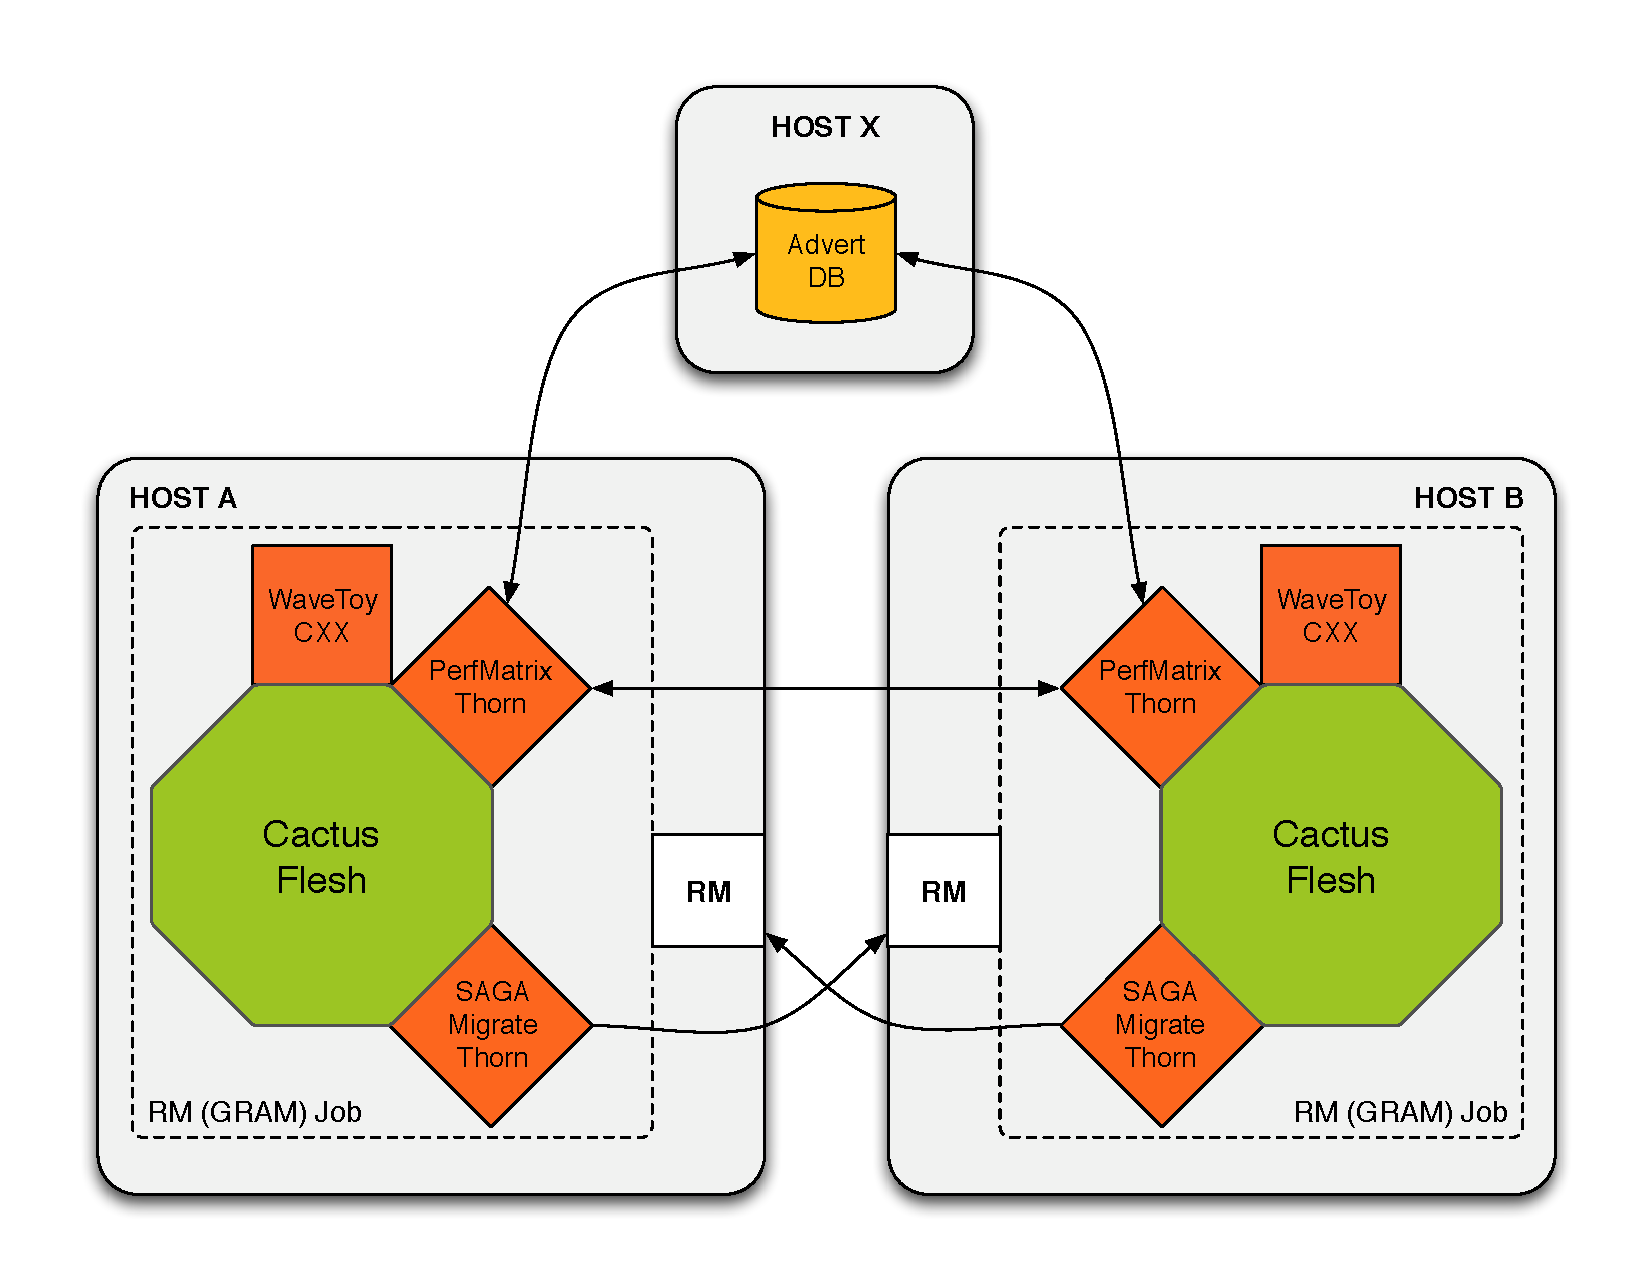
\includegraphics[scale=0.30]{./figures/figure_02}
% \end{center}
% \caption{The components of the application. The Cactus framework orchestrates the \textit{WaveToy} thorn as an example for a distributed calculation, the \textit{NetPerf} thorn for network performance measurement, and the \textit{SAGA Migration} thorn for replication and migration. The \textit{Advert DB}
% stores and archives the measurement results. Note that the application runs under the control of a \textit{Resource Manager (RM)} using SAGA's job management package.}
%  \label{fig:arch}
%  \end{figure}

\subsection { Application Architecture} 
The general architecture of the model application is based on the
programming abstraction provided by the Cactus framework. A set of
thorns that provide specific functionality are orchestrated by the
Cactus flesh as depicted in Fig.~\ref{fig:arch}. The novelty in this
Cactus application is that the complete SAGA API is known by the
Cactus build and deployment system and therewith transparently
accessible from within any thorn. With the SAGA functionality
available it was easy to implement Cactus thorns that can interact
with remote resource mangers (e.g. Globus GRAM2), copy, read, and
write files from and to remote locations (e.g. Globus GridFTP), and
access a remote PostgreSQL based advert service as logging and storage
facility. The properties and implementations of the individual thorns
are described in this section.

\subsubsection{WaveToy} The WaveToy thorn implements the simulation of
a 3D scalar field produced, for example by two orbiting sources.  This
is a simple thorn, but is part of a class of more complex systems,
including Einstein's field equations, Maxwell's or Navier-Stokes
equations.

\subsubsection{PerfMatrix} The PerfMatrix thorn takes care of the
intrinsic network performance measurement and persistent storage of
the results. Currently, the implementation uses
netperf~\cite{netperf_web} to measure unidirectional end-to-end
throughput. Netperf is implemented as a simple client-server model
consisting of two executables:
\begin{itemize}
\item{netserver: the measurement endpoint waiting for incoming connections}
\item{netperf: the initiator of a measurement connecting to a netserver endpoint}
\end{itemize}

The PerfMatrix algorithm uses a list of computational resources which
are potential migration targets for the application. After starting
up, the initial application spawns itself onto all available hosts.
\footnote{This approach is different from the original non-centralised
  spawning scheme shown in Fig.~\ref{fig:algo} The reason for our
  implementation using centralised spawning is the Globus Toolkit's
  (4.0.5) inability of full credential forwarding.} Once all jobs have
been launched, the original spawning application first establishes
netperf connections with all the spawned applications; this is
followed by the spawned applications establishing netperf connections
amongst each other, following the scheme shown in Fig.~\ref{fig:algo}.
The job spawning, control, and I/O redirection is done entirely using
SAGA's job management package.  Once a netperf process returns a
throughput result, the PerfMatrix thorn uses the SAGA advert-service
package to announce the result to a central PostgreSQL database which
is also used as a centralised logging facility. After all netperf
processes have finished and published their results, the database
contains a host-to-host throughput performance matrix along with a
timestamp which is available to other thorns as well as other
applications.

\subsubsection{Advert-service database} SAGA's advert-service package
describes a key-value based hierarchical attribute interface for
storing arbitrary information. The currently available adaptor is
capable to map these structures to an relational SQL schema and store
them in local (SQLite) and remote (PostgreSQL) RDBMS.

SAGA's advert-service offers a convenient way to simplify the
difficult task of centralised data collection and logging within
distributed applications. The advert structure consists of two
hierarchical trees: one for logging (containing the host name, a
timestamp, and the log message) and one for the throughput performance
matrix (containing a timestamp and the matrix itself). Since every
matrix is stored with a timestamp, every time the NetPerf thorn gets
triggered, an additional matrix is added to the advert-service which
leads to a growing stack of time-series data. This time-series can in
turn be analyzed by the SAGAMigrate thorn to determine if and where
to migrate.  Since all data stored in the advert-service can be
directly accessed using SAGA's high-level interface, it is easy to
browse the time-series data from other applications. A simple tool
that generates boxplots (Fig.~\ref{fig:boxplot}) from the performance
matrices is proof of the simplicity.

\subsubsection{SAGAMigrate} The SAGAMigrate thorn is a Cactus thorn
written in C++ that uses SAGA functions (for example file.copy and
job\_description.create\_job) to perform a simulation migration.
SAGAMigrate copies a restart parameter file and the checkpoint file(s)
from one machine to another (for example using the SAGA Globus
adaptors).

% \begin{figure}
%  \begin{center}
%  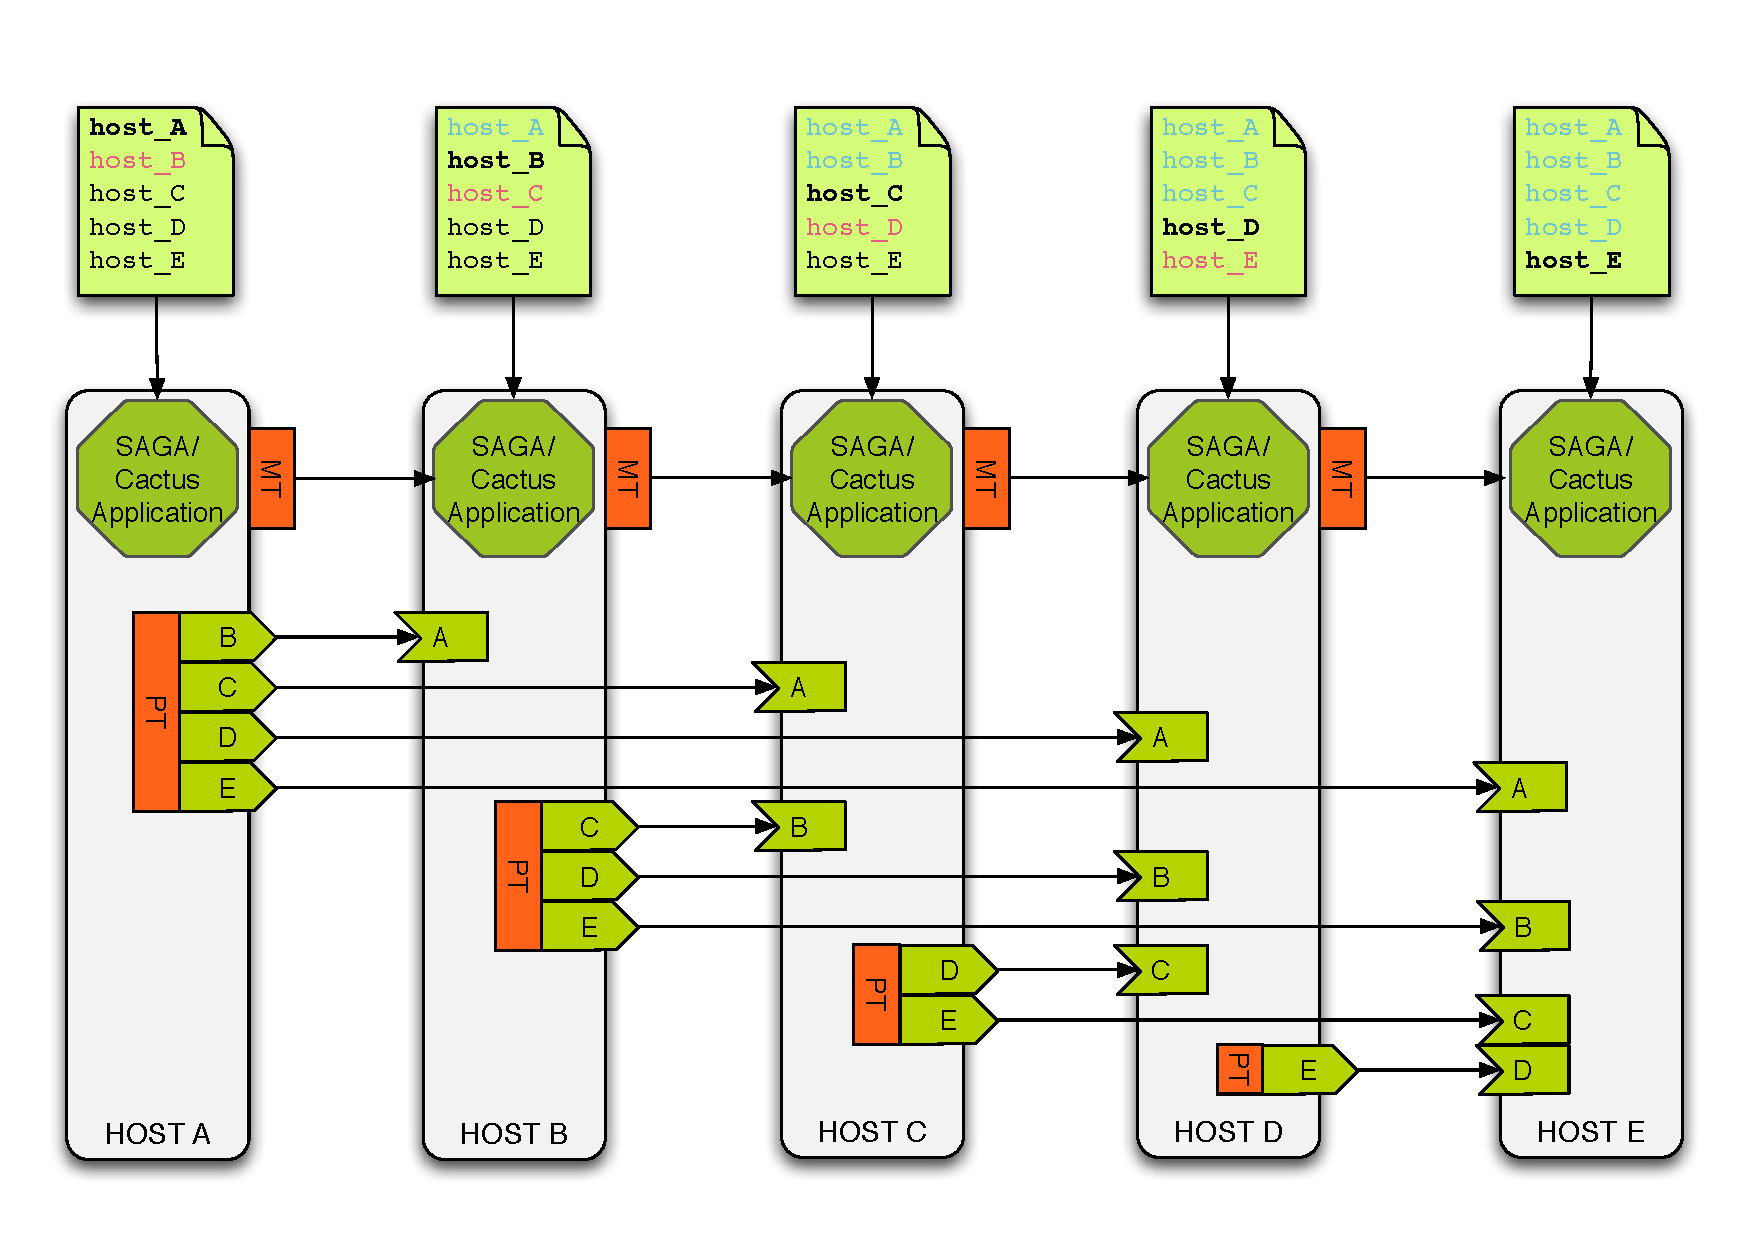
\includegraphics[scale=0.30]{./figures/figure_01}
%  \end{center}
%  \caption{The algorithm used by the PerfMatrix thorn. Based on a list of resources, the application spawns itself, launches Netperf endpoints and measures the throughput of all possible connections. }
%  \label{fig:algo}
%  \end{figure}


\section{Results and Discussion}

% \begin{figure}
% \begin{center}
% 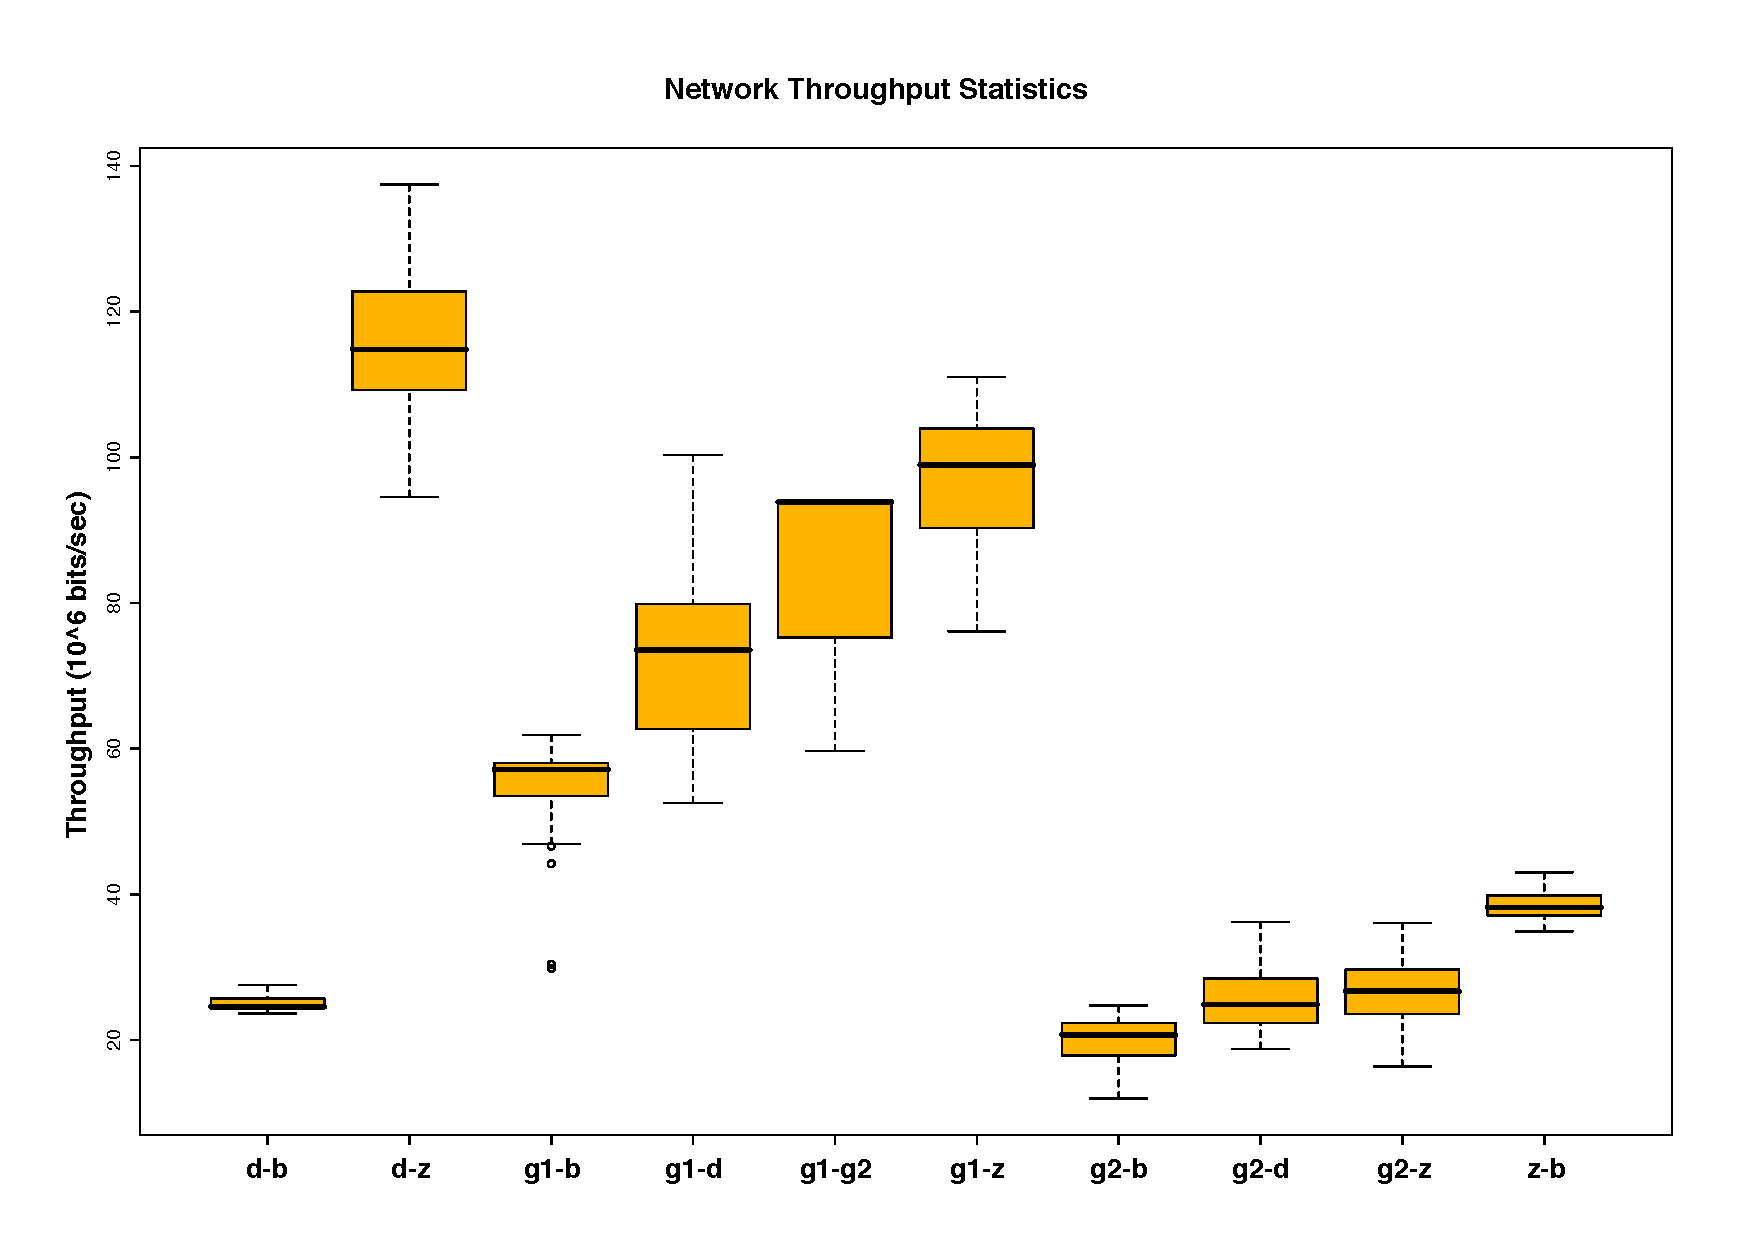
\includegraphics[scale=0.30]{./figures/figure_04}
% \end{center}
% \caption{Network throughput statistics extracted from the advert-service database after running the NetPerf thorn for 12 hours in 10 min. intervals. The letters on the X-axis stand for: d(ucky.loni.org), b(luedawg.loni.org), z(eke.loni.org), g1 (gg101.cct.lsu.edu), g2 (gg201.cct.lsu.edu)}
% \label{fig:boxplot}
% \end{figure}

The SAGAMigrate thorn from WaveToyCXX application parsed data gathered
and based upon that was able to determine which machine to migrate
too. The data gathered over twelve hours at a sampling interval of ten
minutes between the five different resources is shown (using the
Box-and-Whitney format) in Fig~\ref{fig:boxplot}.  As the data
collected shows, our simple application can now serve as a stand-alone
diagnostic tool for networks maintenance and monitoring.  Simple
extensions to the features of the network monitoring thorns, will make
it a full-fledged network diagnostic tool to meet the needs of LONI
for the different use cases discussed in Section II C.

The PerfMatrix thorn provides the capability to use either Time Series
(historical) data or instantaneous real-time data for analysis.  The
ability to collect and analyse both sets is important: for relatively
short-lived transactions real-time data is the more useful information
in order to make placement decisions. For long-time transfers, say of
the order of many terabytes or petabytes, the historical activity is
more relevant, especially if network characteristics are bursty

It is important to mention that similar to solving the computational
job-placement problems (which as alluded to, is a combination of the
job-scheduling and transfer), solving the generalized data-placement
problem -- which in turn is a composition of data-scheduling and
transfer -- is non-trivial.  Current network tests and
parameterizations implemented in the PerfMatrix thorn are simple and,
there are no attempts at dynamical optimization. Advanced modelling
techniques such as Markov-State transition models and others derived
from Queuing Theory are required to solve the complete placement
problem -- for both the data and computational cases as discussed
Sections II C.  It is important to note that whatever the underlying
prediction mechanism or model, it can be encapsulated within a thorn
and used by any application. Arguably for the first time ever, it is
possible to interface different performance and prediction model
directly with the application, and not at the middleware level or
external has been made possible.

A critical feature of this application which arise from using the
correct abstractions (SAGA and Cactus) is {\it the ability to separate
  the computational logic from the distributed logic.}  For example,
jobs on different resources, establish connections pairwise and
collect information which is published to an advert service through
SAGA's job-management package, whilst the PerfMatrix thorn remains
independent of the distributed aspects of the set of netperf
end-points.  Additionally, beyond compiling the application code on
the other resources, there is no need for the application to know
about the details of the middleware/platform of the remote resources.

\section{Future Work and Conclusion}

Our experience should serve as useful input to the community --
resource providers and middleware developer - to support the
development and deployment of SAGA Adaptors.  We created a single set
of Globus adaptors and deployed them on distinct Grids. Our
application successfully utilized these adaptors, without any further
customization, which goes to show that the widespread availability of
SAGA adaptors is an important step towards the creation of distributed
applications that can be universally deployed (i.e.  independent of
the details of the resource's middleware and configuration detail). We
hope to motivate both middleware developers and resource providers
(such as TeraGrid, EGEE, etc.) to subscribe to the SAGA philosophy and
thereby contribute to the development of SAGA adaptors for their
middleware stack as well as deploying these SAGA adaptors.

We also discussed how the deployment of this model application across
two distinct Grids was trivial as it only required the deployment of
of the appropriate SAGA adaptors.  Thus developing both applications
and tools using SAGA is an effective mechanim for ensuring
inter-operability across different middleware distributions -- even at
the application level -- something that is arguably missing in current
Grid Interoperation efforts~\cite{gin_paper}

There are many applications that need to use federated
Grids~\cite{clade06, gin_paper}.  Utilizing SAGA to develop, or at
least provide Grid-functionality is a useful strategy. Therefore, if
the development and deployment of applications across federated grids
is to be facilitated, SAGA adaptor activity -- development and
deployment, needs to be self-sustaining and thus requires explicit
support, from both the middleware developers and resource providers.

The success of e-Science critically depends upon the availability of
e-Infrastructure.  But the promise of e-Science will be hollow without
delivery of the applications and application-enabling paradigms and
technology that can effectively utilize this new infrastructure. We
believe SAGA is an important first step in this direction.

\section{Acknowledgements}

This work has been made possible thanks to the internal resources of
the Center for Computation \& Technology (CCT) at Louisiana State
University.  Important funding for SAGA specification and development
has been provided by the UK EPSRC grant number GR/D0766171/1 (via
OMII).  We would like to acknowledge the support of the OGF SAGA
Research Group for their work towards developing the SAGA
specification (in particular Andre Merzky), as well as the Cactus
team.  Additionally, we would like to acknowledge help from the LONI
support team and CyberInfrastructure Develompent group (CyD) in the
CCT.  We would like to thank Gabrielle Allen for useful input on the
manuscript. Finally, SJ acknowledges the e-Science Institute,
Edinburgh for supporting the theme, ``Distributed Programming
Abstractions''.

\bibliographystyle{IEEEtran}
\bibliography{saga_cactus_escience}

\end{document}

% \jhanote{Two main strands of conclusion: First is the demonstrated
%   ability to develop interesting and novel eScience applications using
%   appropriate abstractions such as SAGA and Cactus.  Second is the
%   specific model application that we have created as proof-of-concept,
%   which although elementary and currently limited, is easily
%   extensible and thus widely usable/required -- as demonstrated in the
%   Use Cases}


% This is a lightweight application, that can be customized to meet
% specific application-level needs. One could in principle modify the
% code to place sensors inside the code which provide data gathering,
% load-balancing etc.. Our approach is different in that this an
% external agent that enables the core application to remain unchanged.
% ``service application''.

% This is an elementary application, but one that establishes the
% advantages of designing Grid-aware applications (or at least
% Grid-functionality of applications) using SAGA.  To do this without
% these appropriately abstracted layers is difficult if not impossible.
% Additionally this ``service application'' can be (i) easily interfaced
% with other legacy applications (as it requires only a (a) SAGA Thorn
% (b) performance thorn), (ii) a wide range of specific performance
% requirements can be accommodated within this framework. 
% Discuss for example, how it is trivial to use this application for the
% scenario in Use Cases 
%...\jhanote{which use case?}

% Development is made easier through the availability of high-level, Grid-primitives. 
% Thus the focus can be on the computational logic and algorithm and not the
% details of implementing the Grid-functionality i.e., marshalling distributed
% resources.
>
